\chapter{Anwendung anhand eines praktischen Beispiels}
\label{ch:prakBsp}
In meinem Fallbeispiel geht es um CloudGEN, einen neuen Ansatz für die verwendung \\ von Generativer KI, in einer adaptiven Cloud Umgebung mit big data. CloudGEN integriert drei Hauptsysteme. Diese Hauptsysteme bestehen aus Monitoring, Training und Integration \\ generativer Modelle zur Datengenerierung gefolgt von einem CNN basiertes \\ Anomalieerkennungssystem. Jedes dieser Module spielt eine zentrale Rolle bei der Neugestaltung der Anomalieerkennungen in Cloud-Umgebungen. Zunächst sammelt das Monitoring-System \\ Rohprotokolldaten aus dem Big-Data-Cluster und speichert diese in einer Zeitreihendatenbank. Als nächstes verfolgt die Komponente Training und Integration die Aufgabe des Trainings und die Bereitstellung von GANs innerhalb von CloudGEN um Deep-Learning-Techniken für eine realistische Datenrepräsentation zu nutzen. Zum Schluss wird das CNN-basierte \\ Anomalieerkennungssystem eingesetzt, um Anomalien innerhalb des cloudbasierten \\ Big-Data-Systems zu identifizieren.\\ Im folgenden Abschnitt werde ich die einzelnen Komponenten näher erläutern ~\cite{Fallbeispiel}.

\\
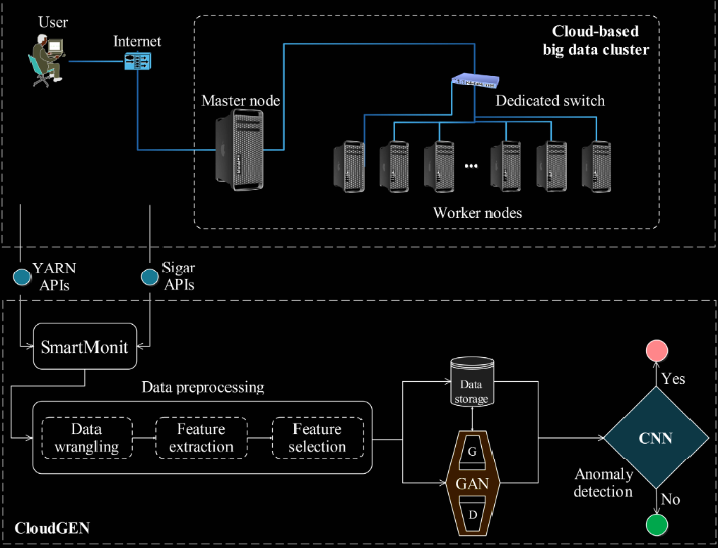
\includegraphics[scale=0.8]{Bilder/CloudGEN.png} Abbildung 1
\\
\\
Die Monitoring-Komponente für die Datenerfassung spielt in CloudGEN eine zentrale Rolle. Sie ist dafür verantwortlich aufkommende Fehlfunktionen oder Leistungsprobleme innerhalb des\\ Big-Data-Systems zu erkennen. Hierbei wird SmartMonit benutzt. SmartMonit ist ein Echtzeit Monitoringsystem für Big Data. Es verfolgt effektiv den Status von Big-Data-Aufgaben und \\ überwacht die Ressourcennutzung in Echtzeit. Es stellt die kontinuierliche Übertragung von \\ Daten von der Quelle in die Zeitreihendatenbank sicher.\nAbsatz Um sämtliche Leistungsmetriken wie die Ausführungszeit, Status, Fortschritt jeder einzelnen Aufgabe sowie Speicherorte der Datenblöcke zu sammeln werden YARN-APIs benutzt. Diese Sammeln diese Metriken vom Masterknoten. Des weiteren werden Metriken zur\\  Ressourcenauslastung wie die CPU Nutzung, Speicherauslastung und Netzwerkverkehr mithilfe von Sigar-Apis erfasst. Die aufgelisteten Metriken werden anschließend an den Consumer \\  übergeben der auf derselben Maschine wie die Datenbank liegt, somit werden die Daten natlos übernommen und in die Datenbank geschrieben. Nachdem alle Daten gesammelt wurden fängt die Datenvorbereitung an, auch Data preprocessing genannt. 
\nAbsatz Die Datenvorbereitung besteht aus drei Schritten. Der erste Schritt ist die Datenbereinigung danach folgt die Merkmalextraktion und zum Schluss eine Merkmalselektion. \\ Die Datenbereinigung auch 'Data Wrangling' genannt dient zur Bereinigung der Daten. \\ Die Rohdaten werden in diesem Schritt umgewandelt und gesäubert, so dass Probleme wie \\ fehlende Werte, Ausreißer und Inkonsistenzen behoben werden und die Integrität des Datensatzes sichergestellt ist. Danach folgt die Merkmalextraktion auch 'Feature Selection' genannt. In diesem Schritt werden aussagekräftige Merkmale extrahiert um relevante Muster für die weitere Analyse zu erfassen und effizient zu nutzen. Der letzte Schritt ist die Merkmalselektion. Dieser Schritt wird auch 'Feature Selection' genannt. Hierbei werden von den Merkmalen aus dem Schritt zuvor die wichtigsten und effektivsten Merkmale in der Entscheidungsphase identifiziert, bevor diese Daten für das Training des GANs benutzt wird. \nAbsatz Die letzte Komponente von CloudGEN ist das Convolutional Neural Network (CNN). Das CNN-basierte Anomalieerkennungssystem ist für die Identifizierung von Anomalien innerhalb des cloudbasierten Big-Data-Systems verantwortlich. Die Implementierung des CNN beginnt mit den vorverarbeiteten Daten, die vom Monitoring-System erzeugt und durch die Komponente \\ Training und Integration generativer Modelle zu Datengenerierung angereichert wurden. \\ Anschließend wird das CNN-Modell auf diesem erweiterten Datensatz trainiert, damit wird sichergestellt dass sowohl reale als auch erzeugte Daten verwendet werden. 
\nAbsatz Zum Schluss möchte ich noch einmal auf die Ergebnisse des Einsatzes von CloudGEN bei der Anomalieerkennung im Bereich eines cloudbasierten Big-Data-Systems eingehen ~\cite{Fallbeispiel}.
\nAbsatz
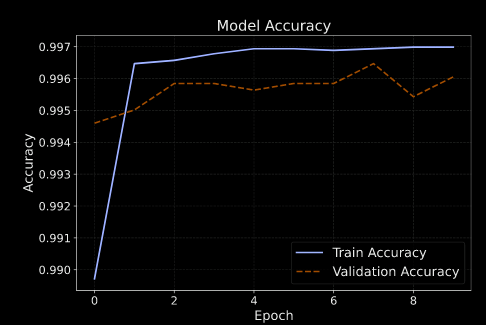
\includegraphics[scale=0.95]{Bilder/ModelAccuracy(9b).png}\\
Abbildung 2
\newpage
\\
Wie im vorhergehenden Diagramm wird dargestellt, wie das Training und die \\ Validierungsgenauigkeit sich über die verschiedenen Epochen entwickelt. Beide Lininen zeigen eine Steigung an, die darauf hinweisen, dass die Genauigkeit konstant ansteigt je mehr Epochen durchlaufen werden. Die Trainingsgenauigkeit scheint sich stetig zu erhöhen und nähert sich \\ nahezu 99,8\%, während die Validierungsgenauigkeit ebenfalls ein ähnliches Muster zeigt, mit leichten Abweichungen ~\cite{Fallbeispiel}.
\nAbsatz
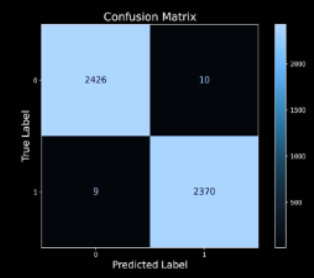
\includegraphics[scale=1.0]{Bilder/Confusion Matrix 10a.png}\\
Abbildung 3
\\
\\
Die Grafik unmittelbar über diesem Textabschnitt zeigt die Leistung des Klassifikationsmodells bei der Unterscheidung zwischen zwei Klassen. Das Modell Klasse 0 bei 2426 Instanzen und Klasse 1 bei 2370 Instanzen korrekt vorhergesagt hat, mit nur 10 falsch-positiven Vorhersagen (Klasse 0 als Klasse 1 vorhergesagt) und 9 falsch-negativen Vorhersagen (Klasse 1 als Klasse 0 vorhergesagt).Die hohe Genauigkeit bei sowohl den wahr positiven und wahr negativen \\ vorhersagen zeigt die Effektivität des Models bei der präzisen Klassifikation der Daten. \\ Des Weiteren möchte ich gerne mit der folgenden Tabelle einen Vergleich der Effektivität im \\ Vergleich zu anderen Modellen zur Anomalieerkennung in Cloud-Computing-Systemen zeigen~\cite{Fallbeispiel}.\\
\\
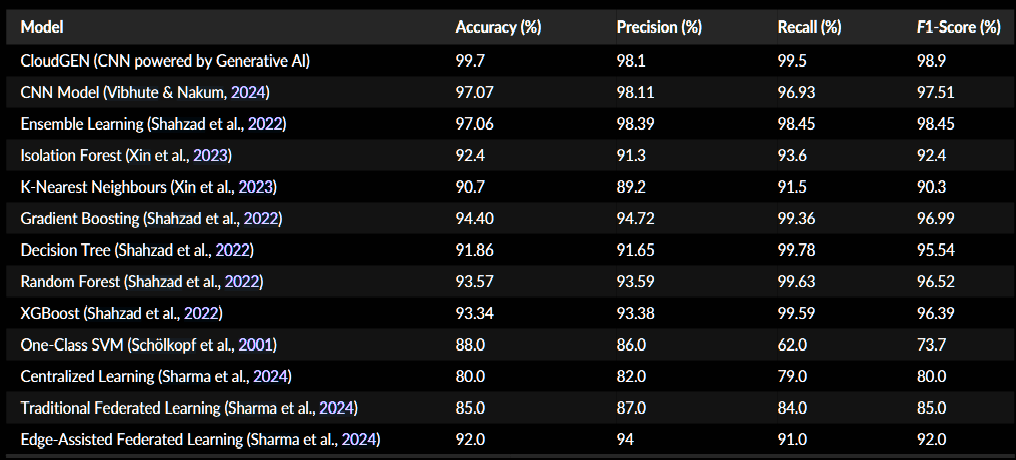
\includegraphics[scale=0.6]{Bilder/ModelleVergleichFallbeispiel table 1.png}\\
Abbildung 4
\\
\\
Diese vergleicht die einzelnen Modelle in den Kategorien: Genauigkeit, Präzision, Recall und dem F1-Score. Unter diesen Kategorien zeigt sich CloudGEN als ein CNN und generatives AI \\ basierendes Modell eine überlegene Leistung in allen Kategorien. Besonders herausragend ist \\ hierbei die Genauigkeit von 99,7\% die noch einmal die Fähigkeit zur Erkennung von \\ Anomalien von CloudGEN zeigt. Durch diese Ergebnisse kann man sehen, dass ein CNN eine effektive Wahl für die Anomalieerkennung in Cloud-Umgebungen ist und die zusätzliche \\ Integration von generativer KI die Leistung noch zusätzlich verbessert. Das zeigt sich vor allem durch die bemerkenswerte Genauigkeit von CloudGEN \cite{Fallbeispiel}.
\nAbsatz
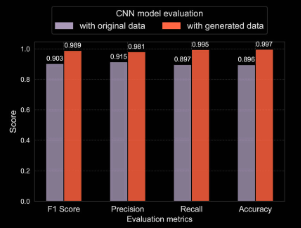
\includegraphics[scale=1.0]{Bilder/Evaluation Matrics 10b.png}\\
Abbildung 5 
\\
\\
In diesem Balkendiagramm werden Bewertungsmetriken wie F1-Score, Präzision, Recall \\ und Genauigkeit für das generative Modell verglichen. Das Modell wird nicht nur auf den \\ Originaldaten evaluiert sondern ebenfalls auf den  generierten Daten. Das auf den generierten \\ Daten bewertete Modell zeigt deutliche Verbesserungen in allen Metriken im Gegensatz zum \\ normalen Modell. Es zeigt sich dass eine Verbesserung von etwa 7\% bis 12\% über alle \\ Kennzahlen besteht. Dies zeigt noch einmal die Wirksamkeit des generativen Modells bei der \\ Verbesserung der Leistungsmetriken des Datensatzes \cite{Fallbeispiel}.
\nAbsatz












